\section{Use Cases Analysis}
\subsection{What? vs How?}
\begin{defBox}[title=Requirements... \enquote{Anforderungen}]
    \begin{itemize}
        \item ...focus on the desired \red{functionality} and \red{operational constraints}
        \item ...are often stated \red{declaratively}
    \end{itemize}
    Perspective of the \red{Client}
\end{defBox}
\begin{defBox}[title=Use Cases... \enquote{Anwendungsfälle}]
    \begin{itemize}
        \item ...identify anticipated \red{interaction} sequences: \red{scenarios}
        \item ...are stated \red{operationally}
    \end{itemize}
    Perspective of the \red{User}
\end{defBox}
\begin{infoBox}
    \begin{itemize}
        \item \fatsf{Anforderungen} beschreiben abstrakt, was das System leisten soll, aus der Perspektive des Kunden, und geben keine Details zur Umsetzung an.
        \item \fatsf{Anwendungsfälle} beschreiben detailliert, wie Benutzer mit dem System interagieren, aus der Perspektive des Benutzers, und sind auf konkrete Abläufe fokussiert.
    \end{itemize}
\end{infoBox}
\begin{figure}[h]
    \centering
    \includegraphics[width=1\textwidth]{Images/What? vs How?.jpeg}
\end{figure}
\subsection{Use Cases: Effort on the Client Side}
\begin{defBox}
    Impossible to write good/complete uses cases without \red{user involvement}
\end{defBox}
\begin{defBox}[title=A Common Misconception]
    Software cost \~ development cost, but in fact:
    \begin{itemize}
        \item Need to allocate at least 30-50\% of development cost \red{at client side} for requirements/use case analysis + validation
        \item Need to allocate ongoing budget for \red{maintenance}
    \end{itemize}
\end{defBox}
\subsection{The CaSh Case Study}
\begin{defBox}[title=Main Roles \& Functionalities (from requirements identification)]
    \blue{General}
    \begin{itemize}
        \item Authentication
    \end{itemize}
    \blue{Administrator}
    \begin{itemize}
        \item Add/change new cars, rental locations
        \item Billing
    \end{itemize}
    \blue{User}
    \begin{itemize}
        \item Check availability
        \item Request booking
        \item \red{Change booking}
    \end{itemize}
    \blue{Service Person}
    \begin{itemize}
        \item Take out vehicle for service
    \end{itemize}
\end{defBox}

\subsection{Text Stories}
\begin{defBox}[title=Change Existing Booking]
    An authenticated customer wants to change an existing booking.\\
    The customer selects the booking to change. The system displays the booking details, including adjacent reservations. The customer is offered to change the reserved duration, or else to cancel the reservation. The customer is offered to change the reserved duration, or else to cancel the reservation.\\
    When a new duration is entered, the system checks availability and records the change. In case of no availability, nothing happens and an information message is displayed.\\
    if the customer chooses to cancel the booking, then it is removed.\\
    Before any change happens, incurred cost is displayed, and a confirmation action is requested. After each change, a confirmation message is sent to the customer's preferred contact.
\end{defBox}
\subsection{Use Cases}
\begin{defBox}
    \begin{itemize}
        \item Use cases are \red{text stories} used to discover and record requirements
        \item Use cases \red{complement} requirements analysis
        \item Use cases provide \red{operational} requirements as a basis for system design
    \end{itemize}
\end{defBox}
\red{Attention:}
\begin{itemize}
    \item Use cases $\neq$ User stories
    \item Use cases are \red{not a replacement} of requirements analysis (do not capture non-functional requirements)
\end{itemize}

\begin{infoBox}
    \begin{itemize}
        \item \fatsf{Use Cases} sind detaillierte Geschichten, die helfen, die \fatsf{Anforderungen zu verstehen} und zu dokumentieren, um später das \fatsf{Systemdesign} darauf aufzubauen.
        \item Sie ergänzen die \fatsf{Anforderungsanalyse} und liefern \fatsf{operative Details}, die als Grundlage für die Entwicklung dienen.
        \item \fatsf{User Stories} sind kürzer und fokussieren sich auf \fatsf{Zielsetzungen}, während \fatsf{Use Cases} konkrete \fatsf{Interaktionsabläufe} detailliert beschreiben.
    \end{itemize}
\end{infoBox}

\subsection{Constituents of Use Cases: Some Definitions}
\red{Actor} Someone or something with \red{behavior}: a person, computer system, an organization, etc.
\begin{itemize}
    \item \red{Primary actor} The actor who requests a service from the system (\blue{initiates} the use case)
\end{itemize}
\red{Scenario} (also known as a \blue{use case instance}) A \red{specific sequence of actions} and interactions between actor and the system
\begin{itemize}
    \item \blue{One} particular story using a system
\end{itemize}
\red{Use case} A \red{collection of} related success and failure \red{scenarios} that describe an actor's usage of a system to achieve a goal

\begin{infoBox}
    \begin{enumerate}
        \item \fatsf{Actor (Akteur)}
        \begin{itemize}
            \item Ein \fatsf{Akteur} ist \fatsf{jemand oder etwas}, das ein Verhalten zeigt und mit dem System interagiert. Das kann eine \fatsf{Person}, ein \fatsf{Computer-System}, eine \fatsf{Organisation} oder sogar ein \fatsf{anderes System sein}.
            \item Der Akteur spielt eine wichtige Rolle in einem Use Case, da er mit dem System interagiert, um ein Ziel zu erreichen. Akteure sind die \enquote{Benutzer} oder \enquote{Stakeholder}, die vom System einen bestimmten Service oder eine Funktionalität anfordern.
        \end{itemize}
        \item Primary Actor (Primäre Akteur)
        \begin{itemize}
            \item Der \fatsf{primäre Akteur} ist der Akteur, der \fatsf{eine Dienstleisung} oder Funktion vom System anfordert und somit den Use Case \fatsf{initiiert}. In den meisten Fällen handelt es sich um den Benutzer, der mit dem System interagiert, aber es kann auch ein anderes System sein, das den Use Case auslöst.
            \item Beispiel: In einem Online-Shop könnte der \fatsf{primäre Akteur} ein \fatsf{Kunde} sein, der ein Produkt kauft.
        \end{itemize}
        \item Scenario (Szenario)
        \begin{itemize}
            \item Ein \fatsf{Szenario (auch als \fatsf{Use Case Instance} bezeichnet) ist eine \fatsf{spezifische Abfolge von Aktionen und Interaktionen} zwischen einem Akteur und dem System. Es beschreibt den Ablauf, wie ein Akteur in einem bestimmten Fall mit dem System interagiert.}
            \item Ein Szenario ist im Grunde genommen eine konkrete \fatsf{Geschichte}, wie der Akteur das System in einer bestimmten Situation nutzt. Es beschreibt, welche Schritte der Akteur ausführt und wie das System darauf reagiert.
            \item Beispiel: Ein Szenario könnte die Schritte beschreiben, die ein Kunde durchführt, um sich in einen Online-Shop einzuloggen und ein Produkt zu kaufen.
        \end{itemize}
        \item \fatsf{Use Case (Anwendungsfall)}
        \begin{itemize}
            \item Ein \fatsf{Use Case} ist eine Sammlung von \fatsf{zusammenhängenden Szenarien}, die den gesamten Ablauf und die verschiedenen Möglichkeiten beschreiben, wie ein Akteur mit einem System interagiert, um ein bestimmtes Ziel zu erreichen.
            \item Der Use Case umfasst sowohl \fatsf{Erfolgsszenarien} (also die Szenarien, in denen das Ziel des Akteurs erfolgreich erreicht wird, möglicherweise aufgrund von Fehlern oder Problemen im System).
            \item Ein Use Case stellt somit eine vollständige \fatsf{Beschreibung des Verhaltens des Systems} dar, das den Akteur bei der Erreichung seines Ziels unterstützt.
            \item Beispiel: Ein Use Case für einen Online-Shop könnte sowohl das Szenario des erfolgreichen Kaufabschlusses als auch Szenarien wie den Abbruch des Kaufs aufgrund einer ungültigen Zahlungsmethode umfassen.
        \end{itemize}
    \end{enumerate}
\end{infoBox}

\subsection{Different Kinds of Use Cases (Other distinctions exist)}
\red{White box vs. Black box} - with whom does interaction take place?
\begin{itemize}
    \item \red{White box} (\enquote{Transparent}) use cases provide a detailed view of \blue{interaction of internals} when satisfying a user goal
    \item \red{Black box} use cases encapsulate the system and describe \blue{only interactions with external actors}
\end{itemize}
\red{Corporate vs. System}
\begin{itemize}
    \item \red{Corporate} (\enquote{geschäftlich}) use cases describe a \blue{business process} (often without mentioning the system under design)
    \item \red{System} use cases are performed and described with respect to the \blue{system under design}
\end{itemize}
\begin{defBox}[title=Defaults]
    \begin{itemize}
        \item Corporate use cases are usually \red{white box} use cases 
        \item System use cases are in their vast majority \red{black box} use cases
    \end{itemize}
\end{defBox}

\subsection{Use Case Formats}
\begin{itemize}
    \item \red{Brief} (\enquote{kurz}) Terse one-paragraph summary, usually main success scenario
    \item \red{\enquote{informell}} Informal paragraph format; multiple paragraphs that cover various scenarios \blue{(as seen above)}
    \item \red{Fully Dressed} (\enquote{ausgearbeitet}) All steps and variations written in detail; there are supporting sections, such as preconditions and success guarantees
\end{itemize}
\begin{infoBox}
    \begin{itemize}
        \item \fatsf{Whitebox vs. Blackbox} unterscheidet, ob interne Abläufe im system sichtbar sind (Whitebox) oder ob nur die externen Interaktionen dargestellt werden (Blackbox).
        \item \fatsf{Corporate vs. System} unterscheidet, ob der Fokus auf einem gesamten Geschäftsprozess liegt (Coporate) oder auf einem System, das entwickelt wird (System).
    \end{itemize}
\end{infoBox}
\begin{defBox}[title=Precision vs. Accuracy (\enquote{Detaillierungsgrad} bzw. \enquote{Zutreffendheit})]
    \red{Precision:} Level of detail provided by the use case description: granularity\\
    \red{Accuracy:} Correctness-is the description of the use case correct for the amount of detail given?
\end{defBox}
\subsection{Template for Fully Dressed Use Case}
\begin{table}[H]
    \centering
    \rowcolors{2}{\thepagecolor}{fgcolor!10!\thepagecolor}
    \renewcommand{\arraystretch}{1.2}
    \begin{tabular}{lll}
        \toprule
        Use Case Section & Purpose/Guidelines \\
        \midrule
        Use Case Name & Start with a verb \enquote{Accomplish this task} \\
        Scope(\enquote{Umfang}) & Corporate, system (better: name), subsystem \\
        Level(\enquote{Ebene}) & Unser goal, summary goal subfunction \\
        Preconditions & What must be true at start \& worth telling the reader\\
        Minimal Guarantee & Fewest promises system makes to stakeholder\\
        Success Guarantee & What must be true on successful completion \& and is worth telling the reader\\
        Main Success Scenario & Representative scenario of successful use case execution\\
        Extensions & Alternative scenarios of success or failure\\
        Terchnologie and Data Variation List & Varying I/O methods and data formats\\
        Frequency of Occurrence & Influences inverstigation, testing and timing of implementation\\
        Miscellaneous & For example, open issues\\
        \bottomrule
    \end{tabular}
\end{table}

\begin{infoBox}[title=Use Case Name]
    \begin{itemize}
        \item Der Name des Use Cases sollte \fatsf{mit einem Verb beginnen} und das Ziel klar formulieren, z.B. \enquote{Abschließen einer Bestellung} oder \enquote{Erstellen eines Benutzerkontos}. Damit wird sofort ersichtlich, \fatsf{welche Aufgabe} der Use Case abdeckt.
    \end{itemize}
\end{infoBox}
\begin{infoBox}[title=Scope(Umfang)]
    \begin{itemize}
        \item Der \fatsf{Umfang} definiert, auf welcher Ebene der Use Case wirkt:
        \begin{itemize}
            \item \fatsf{Corporate:} Unternehmensweit, also ein gesamter Geschäftsprozess.
            \item \fatsf{System:} Ein spezifisches System, das in Entwicklung ist.
            \item \fatsf{Subsystem:} Ein bestimmter Teil eines Systems.
        \end{itemize}
        \item Die Angabe des Umfangs hilft dabei, den Rahmen und die Grenzen des Use Cases klarzustellen.
    \end{itemize}
\end{infoBox}
\begin{infoBox}[title=Level(Ebene)]
    \begin{itemize}
        \item Die Ebene beschreibt den \fatsf{Detaillierungsgrad} des Use Cases:
        \begin{itemize}
            \item \fatsf{User Goal:} Das zentrale Ziel des Benutzers, das den größten Wert liefert.
            \item \fatsf{Summary Goal:} Ein zusammenfassendes Ziel, das \fatsf{mehrere User Goals} abdeckt und den Kontext des Systems beschreibt.
            \item \fatsf{Subfunction:} Eine Funktion, die Teil eines User Goals ist und \fatsf{weiderverwendbar} sein kann.
        \end{itemize}
    \end{itemize}
\end{infoBox}
\begin{infoBox}[title=Preconditions(Vorbedingungen)]
    \begin{itemize}
        \item Die Vorbedingungen beschreiben, \fatsf{was wahr sein muss}, bevor der Use Case beginnen kann.
        \item Sie werden vom System \fatsf{sichergestellt} und \fatsf{nicht während der Ausführung} erneut überprüft. Ein Beispiel wäre, dass der Benutzer bereits angemeldet ist.
    \end{itemize}
\end{infoBox}
\begin{infoBox}[title=Minimal Guarantee (Minimale Garantie)]
    \begin{itemize}
        \item Die Minimalgarantie ist das \fatsf{Mindeste, was das System den Stakeholdern verspricht}, selbst wenn das Hauptziel des Use Cases nicht erreicht wird.
        \item Diese Garantie beschreibt, wie das System in jedem Fall \fatsf{einen Basiswert liefert.} Beispiel: Das System hat alle bisherigen Schritte protokolliert, auch wenn die Bestellung nicht abgeschlossen wurde.
    \end{itemize}
\end{infoBox}
\begin{infoBox}[title=Success Guarantee (Erfolgsgarantie)]
    \begin{itemize}
        \item Die Erfolgsgarantie gibt an, welche \fatsf{Interessen der Stakeholder} nach erfolgreichem Abschluss des Use Cases \fatsf{erfüllt} sein müssen.
        \item Sie ergänzt die Minimalgarantie und wird \fatsf{am Ende des erfolgreichen Hauptszenarios} oder eines alternativen Erfolgspfads definiert. Beispiel: Nach Abschluss ist die Bestellung gespeichert und bestätigt.
    \end{itemize}
\end{infoBox}
\begin{infoBox}[title=Main Success Scenario (Haupt-Erfolgsszenario)]
    \begin{itemize}
        \item Das Haupt-Erfolgsszenario beschreibt die \fatsf{repräsentative Schritt-für-Schritt-Sequenz} eines \fatsf{erfolgreichen Use Case Ablaufs.}
        \item Die Schritte sind \fatsf{nummeriert} und beinhalten die wichtigsten Aktionen, um das Ziel zu erreichen. Der erste Schritt beschreibt oft den \fatsf{Trigger} des Use Cases, also die Aktion, die ihn startet.
    \end{itemize}
\end{infoBox}
\begin{infoBox}[title=Extensions (Erweiterungen)]
    \begin{itemize}
        \item Erweiterungen sind \fatsf{Abweichungen} vom Hauptszenario und beschreiben alternative Pfade oder Fehlerbehandlungen.
        \item Sie beziehen sich \fatsf{eindeutig auf Schritte} im Haupt-Erfolgsszenario, die variieren könnten, und verwenden ein strukturiertes Format:
        \begin{itemize}
            \item Beispiel: Wenn Schritt 2 verändert wird, könnten die Varianten 2.a, 2.b usw. heißen.
            \item Jeder Schritt innerhalb einer Variante ist nummeriert, z.B. 2.a.1 für den ersten Schritt in Variante 2.a.
        \end{itemize}
    \end{itemize}
\end{infoBox}
\begin{defBox}[title=Two fundamental types of scope]
    \begin{itemize}
        \item \red{Design Scope:} \blue{Specified in this row} Defines boundaries of system of the use case (whole corporation, (sub-)system name)
        \item \red{Function Scope} 
        \begin{itemize}
            \item Limits functionality to be realized by system under design 
            \item Managed by a list of functions in and out of scope
        \end{itemize}
    \end{itemize}
\end{defBox}
\begin{defBox}[title=Kinds of goals]
    \begin{itemize}
        \item \red{User goal} \blue{Most important} elementary goal of user that produces value
        \item \red{Summary Goal} Multiple user goals: describes \red{context} of system under design \blue{or} life-cycle \red{sequence} of related goals \blue{or} \red{table of content} for lower-level use cases
        \item \red{Subfunction}
        \begin{itemize}
            \item Use case being \red{part of} a user goal
            \item singled out on a by-need basis, \red{reusable} in multiple goals
        \end{itemize}
    \end{itemize}
\end{defBox}
\begin{defBox}[title=Stakeholder \enquote{Teilhaber}]
    Subject or object with interest in the behavior of the system under design: Company stakeholder, customer, vendor, regulatory agency, ...
\end{defBox}

\subsection{Use Case Extension for CaSh Change Booking}
\begin{defBox}[title=Change Booking]
    When a new duration is supplied, the system checks availability and records the change. In case of no availability, nothing happens and an information message is displayed.\\
    \red{If the given duration isidentical to the reserved period, then nothing happens.}
    Before any change happens, incurred cost in displayed, and a confirmation action is requested.\\
    \red{If the session times out before confirmation is given, nothing happens.}
\end{defBox}

\subsection{Excerpt of Fully Dressed Use Case}
\begin{table}[H]
    \centering
    \rowcolors{2}{\thepagecolor}{fgcolor!10!\thepagecolor}
    \renewcommand{\arraystretch}{1.2}
    \begin{tabular}{lll}
        \toprule
        Use Case Section & Purpose/Guidelines \\
        \midrule
        Name & List Available Cars\\
        Scope & CaSh Booking Module\\
        Level & User goal\\
        Primary Actor & CaSh Customer\\
        Stakeholders and Interests & \red{Customer:} wants to find available cars for a given duration and location.\\
         & \red{CaSh Company:} wants to make accurate offer\\
        Precondition & Customer is authenticated\\
        Minimal guarantee & No side effects\\
        Success guarantee & All available cars of requested class, specified duration, and location are displayed to customer\\
        Main Success Scenario & 1. Customer wants to know whether there is a suitable car to book\\
         & 2. Customer enters address or uses location service;\\
         & enters maximal location distance or use default\\
         & 3. Customer enters desired reservation period\\
         & 4. System validates time period\\
         & 5. Customer completes search details by entering desired class of car\\
         & 6. System determines matching options\\
         & 7. System displays all available cars matching selction criteria\\
          Extensions & 3.a End date is equal to or before start date\\
         & 3.a.1 Ask customer to specify non-empty period\\
         & 5.a Session times out before search details completed\\
         & 5.a.1 Customer is logged out\\
         & 7.a Search criteria give no result\\
         & 7.a.1 System includes cars one class lower and higher\\
         & 7.a.2 System includes cars with partial overlap of requested duration\\
         & 7.a.3 System suggests to customer to increase location distance\\
        \bottomrule
    \end{tabular}
\end{table}

\subsection{Guidelines for Developing Use Cases}
\begin{defBox}[title=In General: Proceed Incrementally]
    \begin{enumerate}
        \item Identify all currently relevant use cases accurately at a \red{very high level}
        \item Add precision \red{gradually}, work out the details
    \end{enumerate}
\end{defBox}

\begin{defBox}[title=Recommended Workflow]
    \begin{enumerate}
        \item List supported \red{acoters} \& their \red{goals}\\
        Review list for accuracy and completeness\\
        \blue{Outcome:} first level of precision of functional requirements
        \item Write \red{stakeholders}, \red{trigger}, and \red{main success scenario} for each use case\\
        \red{Validate} that the system delivers to important stakeholders\\
        \blue{Outcome:} second level of precision for functional requirements
        \item Identify and list all \red{failure conditions}
        \item Write \red{failure handling}\\
        \blue{Do not interleave} this step with the previous one:\\
        Danger of not completing list of all failures
    \end{enumerate}
\end{defBox}

\subsection{Further Recommendations for Writing Use Cases}
\begin{itemize}
    \item During early requirements work: \red{Keep the user interface out} (Focus on \red{intent})
    \item Write \red{terse} use cases
    \item Write \red{black box} use cases: Describe \red{what} the system must do and \red{not how}\\
    For instance:\\
    \enquote{The system records the booking.} (korrekt)
    \enquote{The system writes the booking to a database.} (falsch)
    \item Take an \red{actor} or actor-goal perspective
    \item Focus on the \red{users} or \red{acotors} of a system:
    \begin{itemize}
        \item Ask about their \red{goals} and typical situations
        \item Focus on understanding what the actor considers a \red{valuable result}
    \end{itemize}
\end{itemize}
\begin{defBox}
    Identifying and writing good use cases may take weeks
\end{defBox}

\subsection{Which of these phrases is a valid use case?}
\subsubsection*{Examples}
\begin{itemize}
    \item Negotiate a supplier contact
    \item Handle returned sale
    \item Log in 
    \item Move piece on game board
\end{itemize}

\subsubsection*{Checklist}
\begin{itemize}
    \item Is it a well-defined \red{task} ...
    \begin{itemize}
        \item performed by \red{one stakeholder} in one place at one time,
        \item to model a \red{business event}, 
        \item which \red{adds measurable business value} and
        \item leaves the data in a \red{consistent state}?
    \end{itemize}
    This is called \red{Elementary Business Process (EBP)}
    \item Is it not merely a single step (\blue{size test})?
\end{itemize}

\begin{defBox}[title=Which of these phrases is a valid use case?]
    \begin{itemize}
        \item Negotiate a supplier contract: (no) too complex-no \red{elementary} business case
        \item Handle retruned sale: (yes)
        \item Log in: (no) Depends on context, usually does not add value to business case
        \item Move piece on game board: (no) Single step, fails size test
    \end{itemize}
\end{defBox}

\section{UML Use Case Diagrams}
\subsection{The Unified Modeling Language (UML)}
\begin{defBox}[title=Some Facts]
    \begin{itemize}
        \item The Unified Modeling Language (UML) is a \red{visual}, yet precise, \red{design notation} for software development
        \item Originated as merger of the three OO modelling approaches: \blue{Booch, OMT, OOSE}- as well as best practices
        \item Maintained and developed by the Object Modeling Group (OMG)
        \item Main \red{goal}: support object modelling \red{tool interoperability} by agreeing on syntax and semantics of underlying modelling language
        \item Consists of collection of \red{diagrammatic modelling notations}, including:
        \begin{itemize}
            \item \red{Use case} diagram
            \item \red{Class}, object, package diagram
            \item Sequence, collaboration, activity diagram
            \item \red{State} diagram, ... + ca. 10 more
        \end{itemize}
    \end{itemize}
\end{defBox}
\begin{infoBox}[title=Sammlung von diagrammatischen Modellierungsnotationen:]
    \begin{itemize}
        \item UML besteht aus \fatsf{verschiedenen Diagrammtypen}, die unterschiedliche Aspekte eines Systems abbilden. Die gängigsten UML-Diagramme sind:
        \begin{itemize}
            \item \fatsf{Use Case Diagram:} Zeigt die Interaktionen zwischen dem System und seinen Akteuren.
            \item \fatsf{Class Diagram:} Stellt die Klassenstruktur eines Systems dar und zeigt Beziehungen zwischen Klassen.
            \item \fatsf{Object Diagram:} Zeigtdie Instanzen von Klassen zu einem bestimmten Zeitpunkt und deren Beziehungen.
            \item \fatsf{Package Diagram:} Organisiert Klassen und andere Elemente in Gruppen.
            \item \fatsf{Sequence Diagram:} Stellt die zeitliche Reihenfolge der Interaktionen zwischen Objekten dar.
            \item \fatsf{Collaboration Diagram:} Zeigt, wie Objekte miteinander kommunizieren, um eine Aufgabe zu erfüllen.
            \item \fatsf{Activity Diagram:} Stellt Workflows und Aktivitäten in einem Prozess dar.
            \item \fatsf{State Diagram:} Beschreibt die Zustände eines Objekts und die Übergänge zwischen diesen Zuständen.
        \end{itemize}
        \item Insgesamt umfasst UML rund \fatsf{14 verschiedene Diagrammtypen}, die verschiedene Aspekte eines Systems abdecken.
    \end{itemize}
\end{infoBox}
\begin{infoBox}
    UML ist eine \fatsf{standardisierte Modellierungssprache}, die aus mehreren Diagrammtypen besteht und speziell entwickelt wurde, um \fatsf{objektorientierte System visuell zu modellieren.} Sie erleichtert das Design komplexer Systeme, indem sie eine klare, visuelle und universelle Noatation für Entwicklerteams weltweit bietet.
\end{infoBox}

\subsection{UML Use Case Diagram}
\begin{figure}[h]
    \centering
    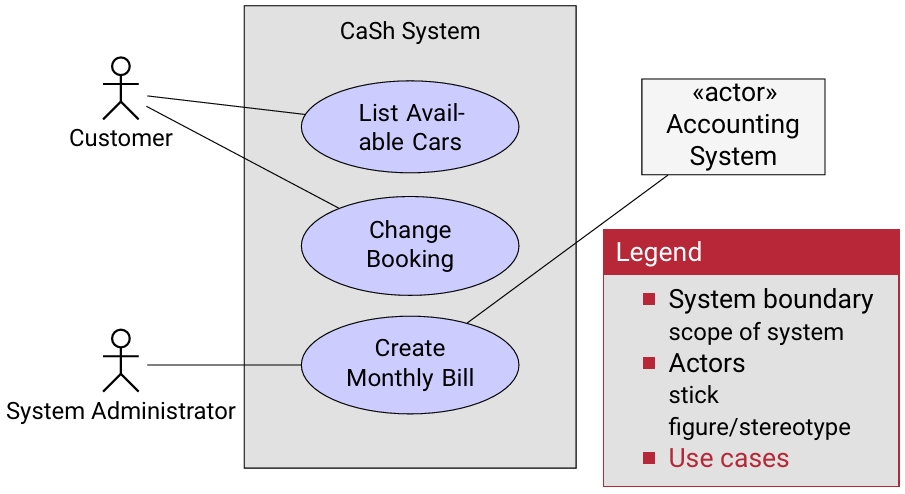
\includegraphics[width=1\textwidth]{Images/UML Use Case Diagram.jpeg}
\end{figure}

\subsection{Remarks on UML Use Case Diagrams}
\begin{itemize}
    \item UML use case diagram notation is intentionally \red{minimalist}
    \item UML use case diagrams are \red{organizational method} to improve
    \begin{itemize}
        \item communication and comprehension of use cases
        \item to reduce text duplication
    \end{itemize}
\end{itemize}
\begin{defBox}
    Organizing use cases into relationships has no impact on the behavior or requirements of a system
\end{defBox}
\begin{itemize}
    \item Use case diagrams provide a \red{black-box view} on a software system
    \item Use case diagrams are helpful only during \red{early} phase of use case analysis
\end{itemize}
\begin{itemize}
    \item \blue{Unsuitable to represent fully dressed use cases}
\end{itemize}

\clearpage
\subsection{The UML Use Case <<include>> Relation}
\begin{figure}[h]
    \centering
    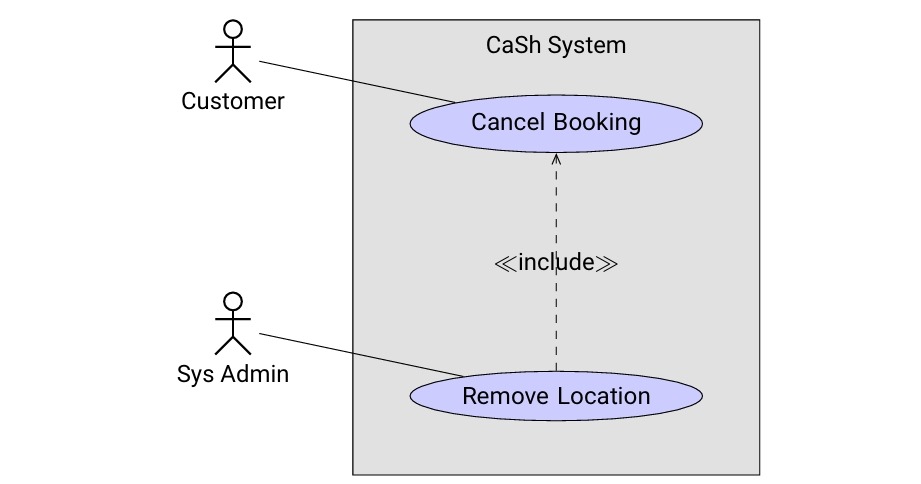
\includegraphics[width=1\textwidth]{Images/The UML Use Case include Relation.jpeg}
\end{figure}
\begin{defBox}[title=Include Relation]
    Factor out \red{common behaviour} across several use cases into its own sub-function use case and indicate inclusion\\
    \red{Facilitates decomposition of large use cases and enables reuse}
\end{defBox}
\begin{defBox}
    Included use cases are always executed
\end{defBox}
\begin{infoBox}
    Die \fatsf{<<include>>-Beziehung} in UML-Anwendungsfalldigrammen dient dazu, \fatsf{gemiensames Verhalten aus mehreren Anwendungsfällen herauszulösen} und in einem eigenen \fatsf{Unteranwendungsfall} (Sub-Use-Case) zu definieren. Diese Vorgehensweise ermöglicht eine klare Struktur und Wiederverwendbarkeit.
\end{infoBox}

\clearpage
\subsection{The UML Use Case <<extend>> Relation}
\begin{figure}[h]
    \centering
    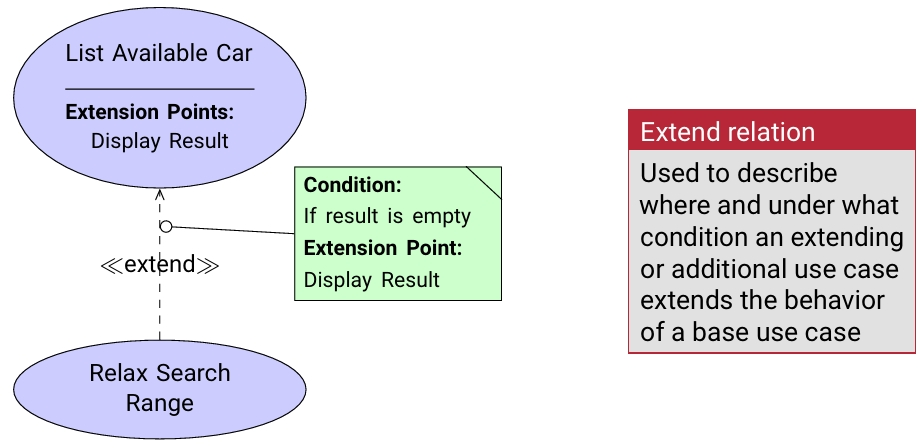
\includegraphics[width=1\textwidth]{Images/extend Relation.jpeg}
\end{figure}
\begin{infoBox}
    Die <<extend>>-Beziehung wird genutzt, um \fatsf{zusätzlich Funktionalität} zu beschreiben, die nur unter bestimmten Bedingungen in einem Anwendungsfall ausgeführt wird. Dies ist hilfreich, wenn:
    \begin{itemize}
        \item Ein Anwendungsfall durch eine zusätzliche Funktionalität ergänzt werden soll, aber diese Funktionalität \fatsf{nur unter bestimmten Bedingungen} ausgeführt werden muss.
        \item Die <<extend>>-Beziehung \fatsf{nur dann aktiviert wird}, wenn eine Bedingung erfüllt ist.
        \item \fatsf{Beispiel:} In einem Autovermietungssystem könnte der Anwendungsfall \fatsf{\enquote{Verfügbare Autos anzeigen}} surch einen \fatsf{\enquote{Suchbereich erweitern}}-Anwendungsfall ergänzt werden. Wenn keine Autos gefunden werden, könnte die Funktion automatisch die Suchkriterien erweitern, um alternative Autos zu finden.
    \end{itemize}
\end{infoBox}

\subsection{Remarks on UML Use Case <<extend>> Relation}
\begin{defBox}[title=Original Intention]
    Extension use cases allow to \enquote{modularly} extend existing use cases \red{But violated by need for explicit extension points in UML use cases!}
\end{defBox}
\begin{itemize}
    \item Most extensions in fully dressed use cases \red{do not} qualify as separate use case (\red{no EBP})
    \item In general (not only UML) extension use cases \red{expose internals} of base use case (in UML even enforced by extension points)
\end{itemize}
\begin{defBox}
    \red{<<extend>>} relation in use case diagrams only when \red{really} justified
\end{defBox}
\begin{infoBox}
    \begin{itemize}
        \item \fatsf{Modularität:} Ursprünglich gedacht, um existierende Anwendungsfälle modular zu erweitern.
        \item \fatsf{Verletzung der Kapselung:} Die Erweiterungspunkte (<<extension points>>) in UML erfordern es oft, dass interne Details des Basissystems offengelegt werden. Daher sollte die <<extend>>-Beziehung nur dann verwendet werden, wenn die Erweiterung wirklich gerechtfertigt ist.
    \end{itemize}
\end{infoBox}

\clearpage
\subsection{UML Use Case Inheritance (Merely for Completeness, Do Not Use!)}
\begin{figure}[h]
    \centering
    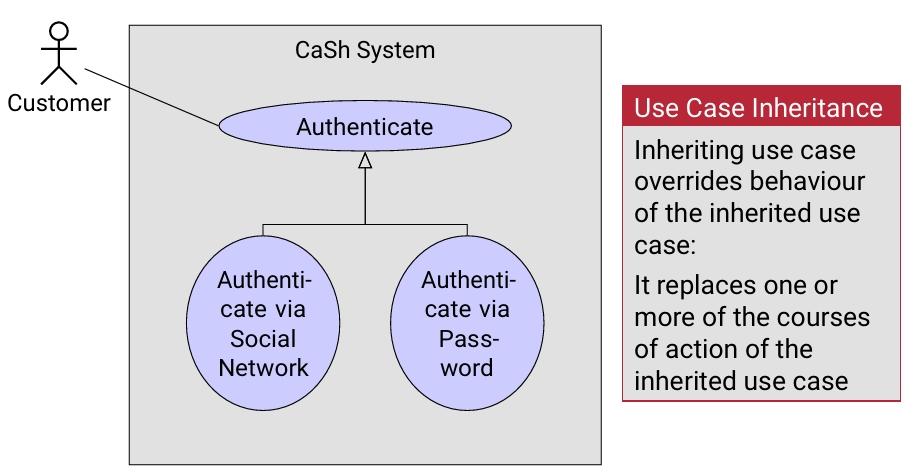
\includegraphics[width=1\textwidth]{Images/UML Use Case Inheritance.jpeg}
\end{figure}

\subsection{Use Cases: Final Remarks}
\begin{defBox}
    Biggest danger: Abusing use cases for system design
\end{defBox}
\begin{itemize}
    \item Use cases are in the \red{problem space.} They document behavioral requirements, \red{use involvement} essential.
    \item Adequate \red{granularity} is important: \red{Elementary business process}, not just a step
    \item \blue{UML use diagrams} most helpful in early use case analysis
    \begin{itemize}
        \item Stay simple, \red{black box} preferred
        \item \red{<<extend>>} breaks encapsulation, use only when justified in UML diagrams 
        \item Never try to anticipate system design with use cases - Don't use \red{inheritance} in UML use case diagrams
        \item Use \red{template}, not diagrams, for fully dressed use case
    \end{itemize}
\end{itemize}